\tikzstyle{block} = [rectangle, minimum width=2cm, minimum height=1cm,text centered, draw=black]
\tikzstyle{block_1} = [rectangle, minimum width=2cm, minimum height=1cm,text centered, draw=black, fill=blue!5]
\tikzstyle{block_2} = [rectangle, minimum width=2cm, minimum height=1cm,text centered, draw=black, fill=red!5]
\tikzstyle{arrow} = [thick,->,>=stealth]
\tikzstyle{arrow_2} = [very thick,->,>=stealth]
\tikzstyle{arrow_3} = [thick,->,>=stealth,dashed]
\tikzstyle{pfr} = [cylinder, draw, minimum height=4cm, minimum width=1cm, shape aspect=1, shape border rotate=180]
\usetikzlibrary{shapes.geometric}


\newpage
\section*{FIGURES}

\begin{figure}[!htbp]
    \centering
    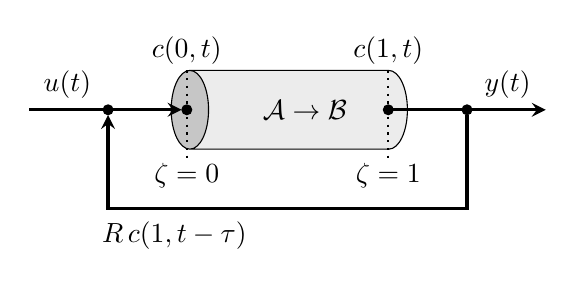
\begin{tikzpicture}
        \node (pfr) [cylinder, draw, minimum height=3cm, minimum width=1cm, shape aspect=1, shape border rotate=180, cylinder uses custom fill, cylinder end fill=gray!45, cylinder body fill=gray!15] {$\mathcal{A} \rightarrow \mathcal{B}$};
        \node (pfr_inlet) [circle, left of=pfr, xshift=-0.5cm, fill=black, draw, inner sep=0pt, minimum size=0.25cm, scale=0.5] {};
        \node (pfr_outlet) [circle, at={(pfr.east)}, shift={(-0.25cm,0)}, fill=black, draw, inner sep=0pt, minimum size=0.25cm, scale=0.5] {};
        \node (recycle_right) [circle, right of=pfr_outlet, fill=black, draw, inner sep=0pt, minimum size=0.25cm, scale=0.5] {};
        \node (recycle_left) [circle, left of=pfr_inlet, fill=black, draw, inner sep=0pt, minimum size=0.25cm, scale=0.5] {};
    
        \draw[dotted, thick] ([yshift=0.5cm]pfr_inlet.center) -- node[at end, below, yshift=0.1cm] {$\zeta = 0$} ([yshift=-0.65cm]pfr_inlet.center);
        \draw[dotted, thick] ([yshift=0.5cm]pfr_outlet.center) -- node[at end, below, yshift=0.1cm] {$\zeta = 1$} ([yshift=-0.65cm]pfr_outlet.center);
    
        \node[below of=recycle_left, node distance=1.3cm, anchor=north west, xshift=-0.2cm] {$R \, c(1, t-\tau)$};
        \node[above of=pfr_inlet, node distance=0.75cm,] {$c(0, t)$};
        \node[above of=pfr_outlet, node distance=0.75cm,] {$c(1, t)$};
        
        \draw [arrow_2] (pfr_outlet) -- node[near end, above] {$y(t)$} ++(2,0);
        \draw [arrow_2] (pfr_inlet) ++(-2,0) coordinate(start) -- node[near start, above] {$u(t)$} (pfr_inlet);
        \draw [arrow_2] (recycle_right) -- ++(0,-1.25) -| (recycle_left);
        
    \end{tikzpicture}
    \caption{Axial tubular reactor with recycle stream.}
    \label{fig:reactor_scheme}
\end{figure}

% \begin{figure}[!htbp]
%     \centering
%     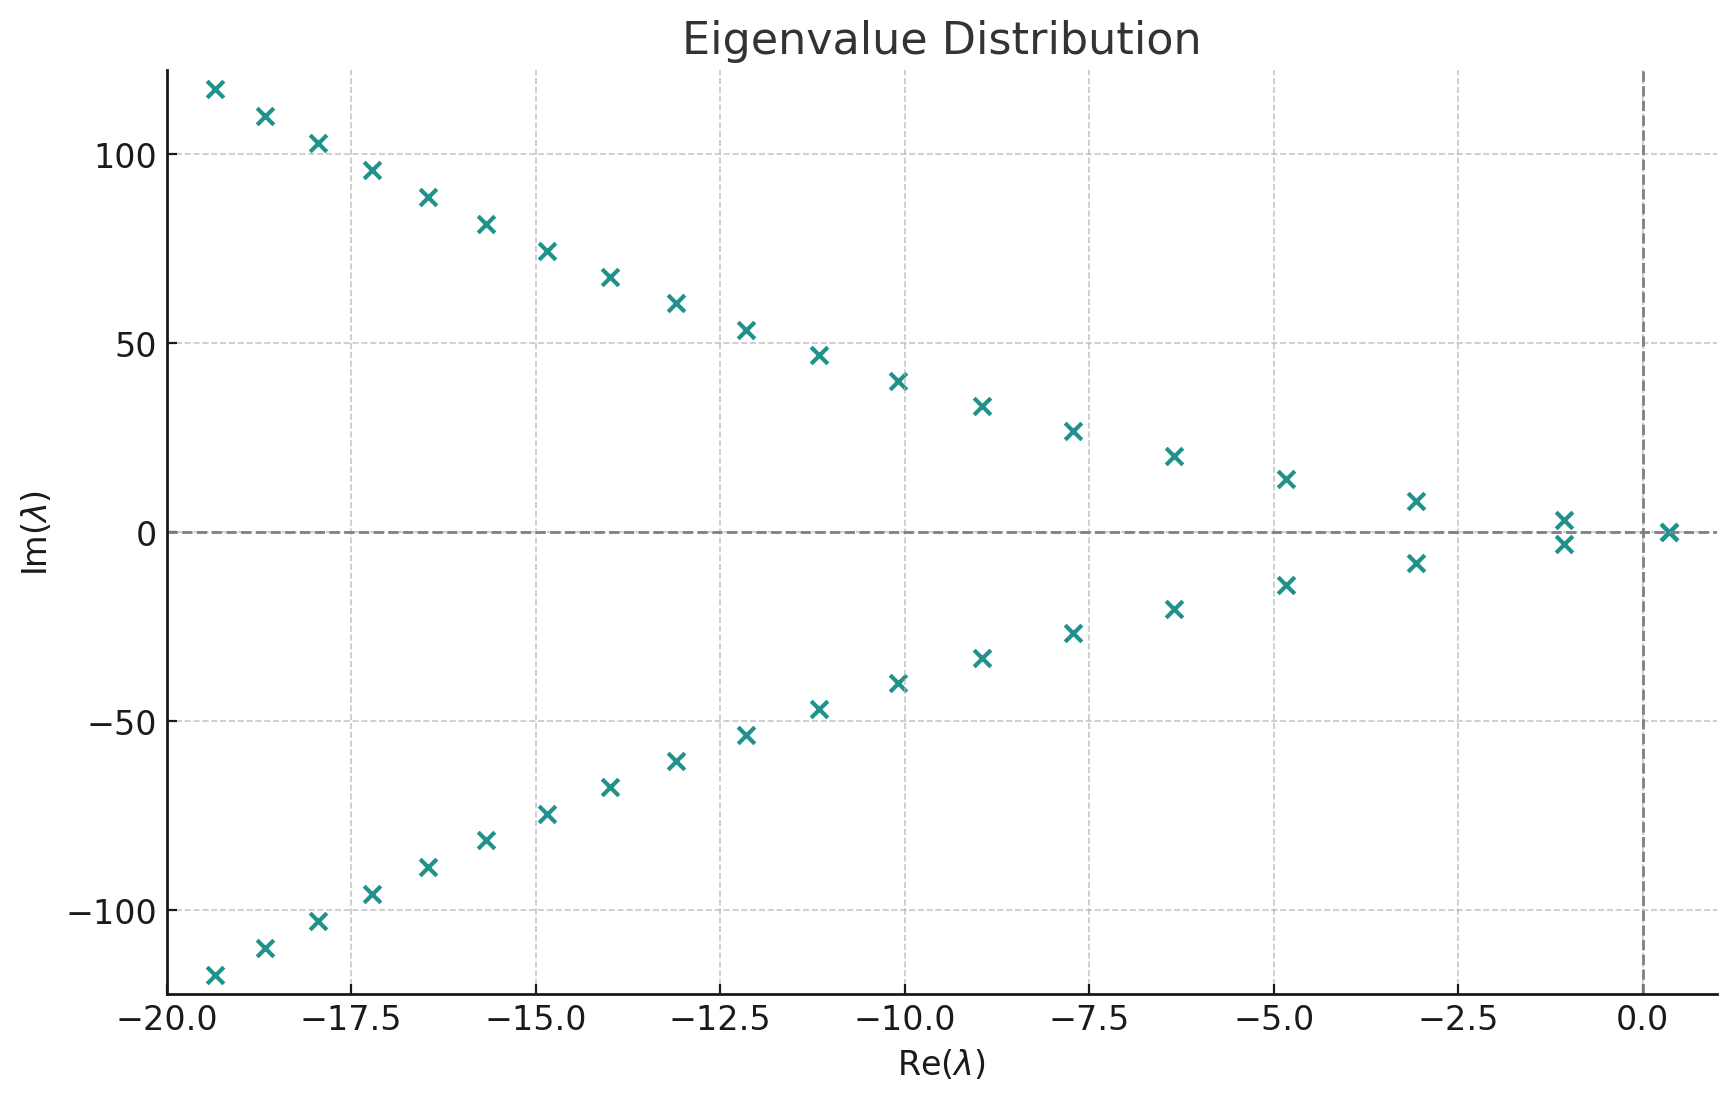
\includegraphics[width=0.7\textwidth]{Figures/eigval_dist_R_0.3.jpg}
%     \caption{Eigenvalues of operator $\mathfrak{A}$ obtained by solving Equation~(\ref{eq:eigval_calc_4}).}
%     \label{fig:eigval_dist}
% \end{figure}

\begin{figure}[!htbp]
    \centering
    \includesvg[inkscapelatex=false, width=0.8\textwidth, keepaspectratio]{Figures/eig_val_dist_R_0.3.svg}
    \caption{Eigenvalues of operator $\mathfrak{A}$ obtained by solving Equation~(\ref{eq:eigval_calc_4}).}
    \label{fig:eigval_dist}
\end{figure}

% \begin{figure}[!htbp]
%     \centering
%     \includesvg[inkscapelatex=false, width=0.8\textwidth, keepaspectratio]{Figures/eigval_dist_R_0.3.svg}
%     \caption{Eigenvalues of operator $\mathfrak{A}$ obtained by solving Equation~(\ref{eq:eigval_calc_4}).}
%     \label{fig:eigval_dist}
% \end{figure}

\begin{figure}[!htbp]
    \centering
    \includesvg[inkscapelatex=false, width=0.6\textwidth, keepaspectratio]{Figures/eigfuns.svg}
    \caption{First few eigenmodes of $\mathfrak{A}$ and $\mathfrak{A}^*$.}
    \label{fig:eigfun}
\end{figure}

\begin{figure}[!htbp]
    \centering
    \begin{subfigure}[b]{0.45\textwidth}
        \centering
        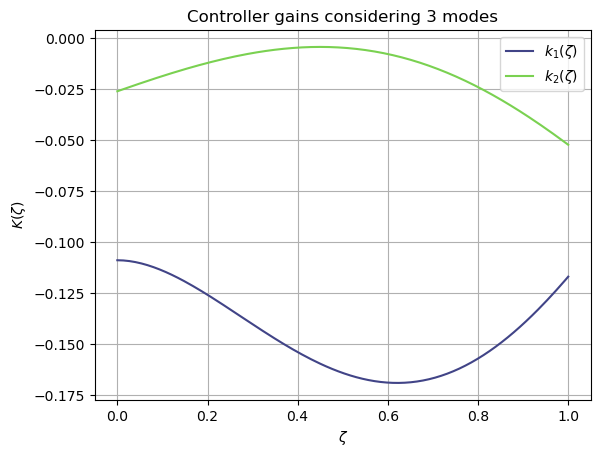
\includegraphics[width=\textwidth]{Figures/k_3.png}
        \caption{$N = 3$}
        \label{fig:k_3}
    \end{subfigure}
    \hfill
    \begin{subfigure}[b]{0.45\textwidth}
        \centering
        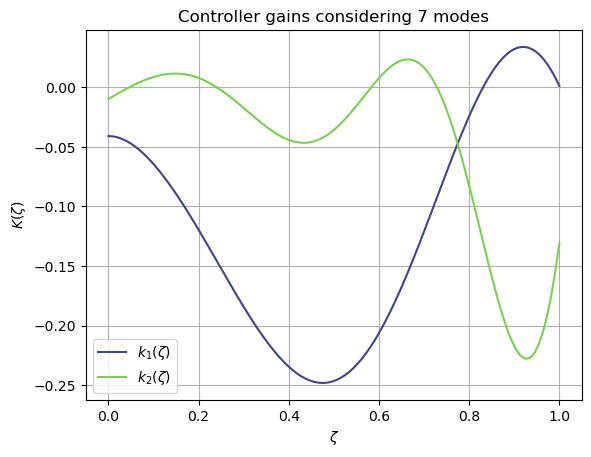
\includegraphics[width=\textwidth]{Figures/k_7.png}
        \caption{$N = 7$}
        \label{fig:k_7}
    \end{subfigure}
    \caption{Full-state feedback gain $\bm{K}(\zeta)$ utilizing the first $N$ modes of the system given by Equation~(\ref{eq:fullstate_gain}).}
    \label{fig:k_modes}
\end{figure}

\begin{figure}[!htbp]
    \centering
    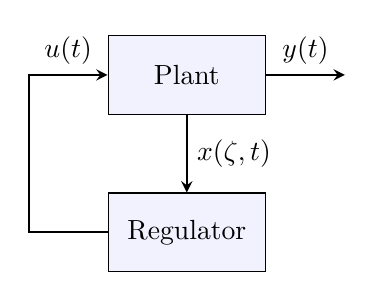
\begin{tikzpicture}[node distance=2cm]
        \node (plant) [block_1] {Plant};
        \node (regulator) [block_1, below of=plant] {Regulator};
        \draw [arrow] (plant.south) -- node[midway, right] {$\bm{x}(\zeta,t)$} (regulator.north);
        \draw [arrow] (regulator.west) -- ++(-1,0) |- node[near end, above] {$u(t)$} (plant.west);
        \draw [arrow] (plant.east) -- node[midway, above] {$y(t)$} ++(1,0);
    \end{tikzpicture}
    \caption{Block diagram representation of the optimal full-state feedback control system.}
    \label{fig:block_diagram}
\end{figure}

\begin{figure}[!htbp]
    \centering
    \includesvg[inkscapelatex=false, width=0.5\textwidth, keepaspectratio]{Figures/L.svg}
    \caption{Observer gain $\bm{L}(\zeta)$.}
    \label{fig:L_modes}
\end{figure}

\begin{figure}[!htbp]
    \centering
    \includesvg[inkscapelatex=false, width=0.5\textwidth, keepaspectratio]{Figures/pole_placement.svg}
    \caption{Eigenvalues of the observer-based controller, full-state feedback controller, and open-loop system.}
    \label{fig:eigs}
\end{figure}

\begin{figure}[!htbp]
    \centering
    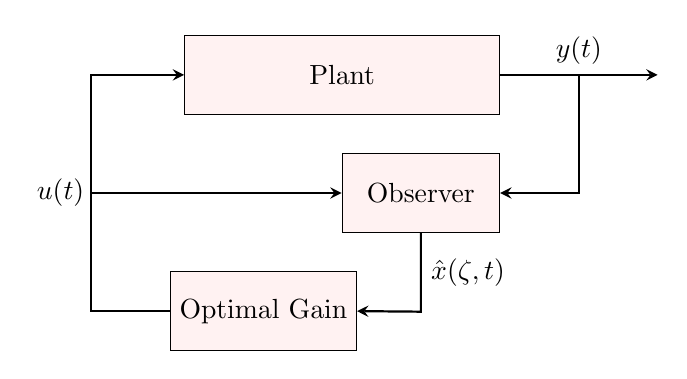
\begin{tikzpicture}[node distance=2cm]
        \node (plant) [block_2, minimum width=4cm] {Plant};
        \node (regulator) [block_2, below of=plant, xshift=-1cm, yshift=-1cm] {Optimal Gain};
        \node (observer) [block_2, below of=plant, xshift=1cm, yshift=0.5cm] {Observer};
        \draw [arrow] (plant.east) -- node[midway, above] {$y(t)$} ++(2,0);
        \draw [arrow] (plant.east) ++(1,0) |- (observer.east);
        \draw [arrow] (observer.south) -- ++(0,-1) node[midway, right] {$\hat{\bm{x}}(\zeta,t)$} -- (regulator.east);    
        \draw [arrow] (regulator.west) -- ++(-1,0) |- (plant.west);
        \draw [arrow] (regulator.west) ++(-1,1.5) coordinate(start) -- node[near start, left, xshift=-0.75cm] {$u(t)$} (observer.west);
    \end{tikzpicture}
    \caption{Block diagram representation of the observer-based output feedback control system.}
    \label{fig:block_diagram_observer}
\end{figure}

\begin{figure}[!htbp]
    \centering
    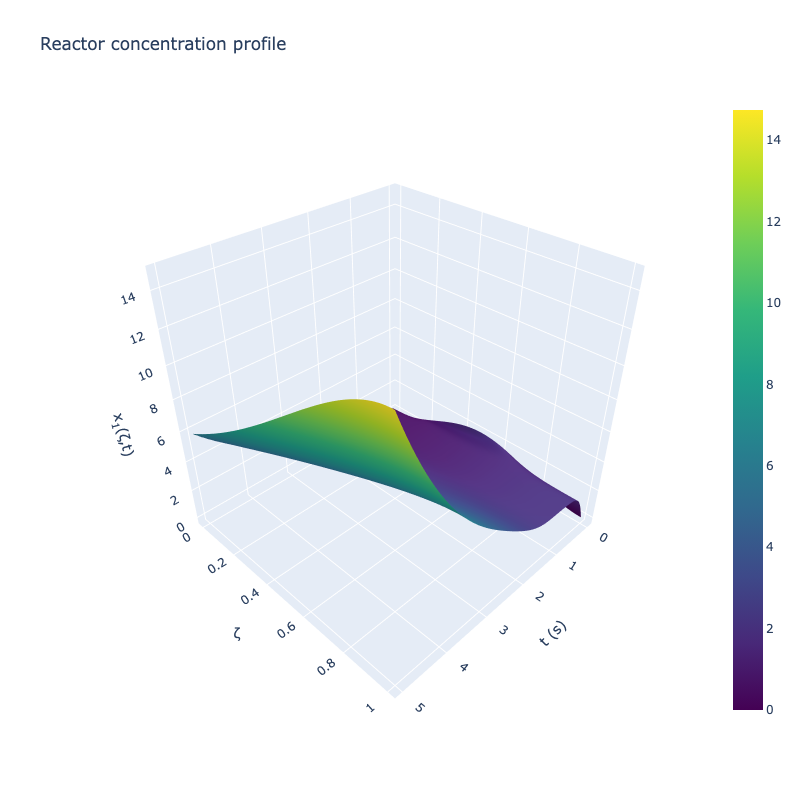
\includegraphics[width=0.8\textwidth,trim=0 0 100 0,clip]{Figures/3D_x1_openloop.png}
    \caption{Zero-input response of the unstable open-loop system as described by Equations~(\ref{eq:PDE_original_model})~and~(\ref{eq:BC}).}
    \label{fig:3D_x1_openloop}
\end{figure}

\begin{figure}[!htbp]
    \centering
    \begin{subfigure}[b]{0.45\textwidth}
        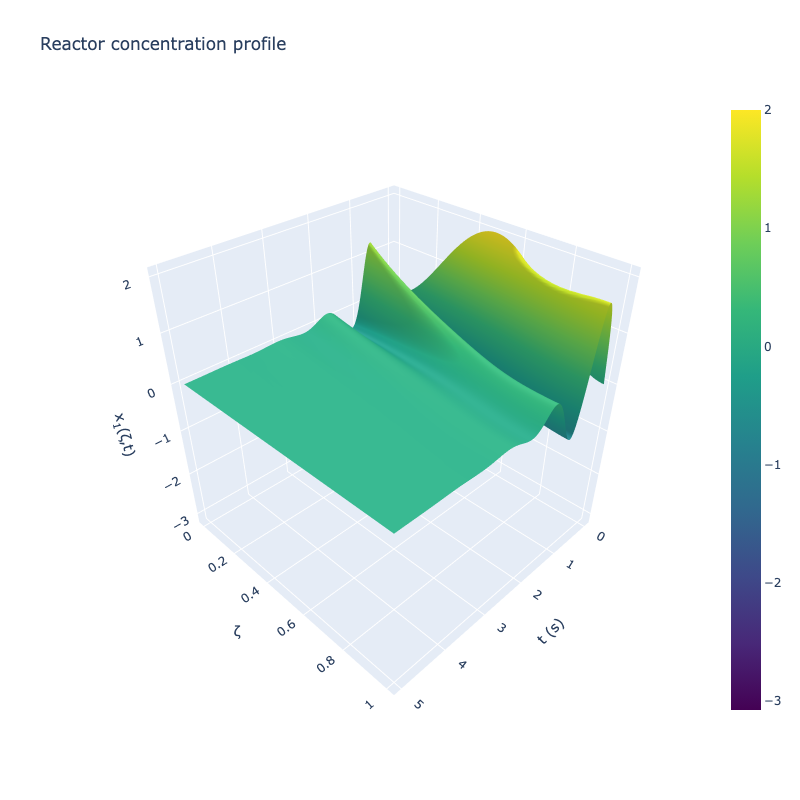
\includegraphics[width=\textwidth,trim=0 0 100 0,clip]{Figures/3D_x1_k3.png}
        \caption{$N=3$}
        \label{fig:3D_x1_k3}
    \end{subfigure}
    \hfill
    \begin{subfigure}[b]{0.45\textwidth}
        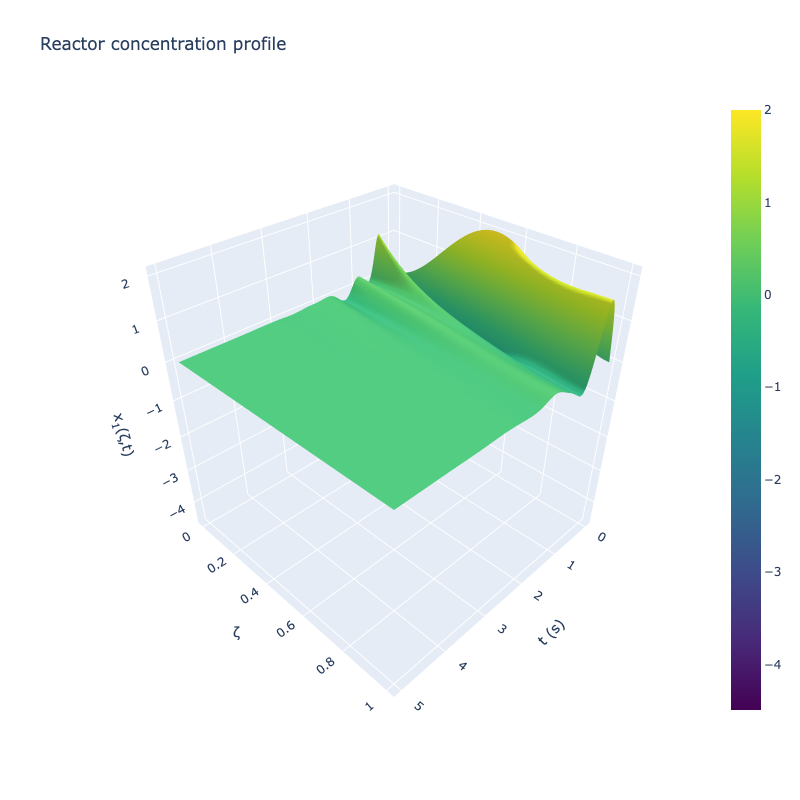
\includegraphics[width=\textwidth,trim=0 0 100 0,clip]{Figures/3D_x1_k7.png}
        \caption{$N=7$}
        \label{fig:3D_x1_k7}
    \end{subfigure}
    \caption{Input response of the system under full-state feedback control given by Equation~(\ref{eq:fullstate_ss}), utilizing the feedback gain obtained in Figure~\ref{fig:k_modes}.}
    \label{fig:full_state_feedback}
\end{figure}

\begin{figure}[!htbp]
    \centering
    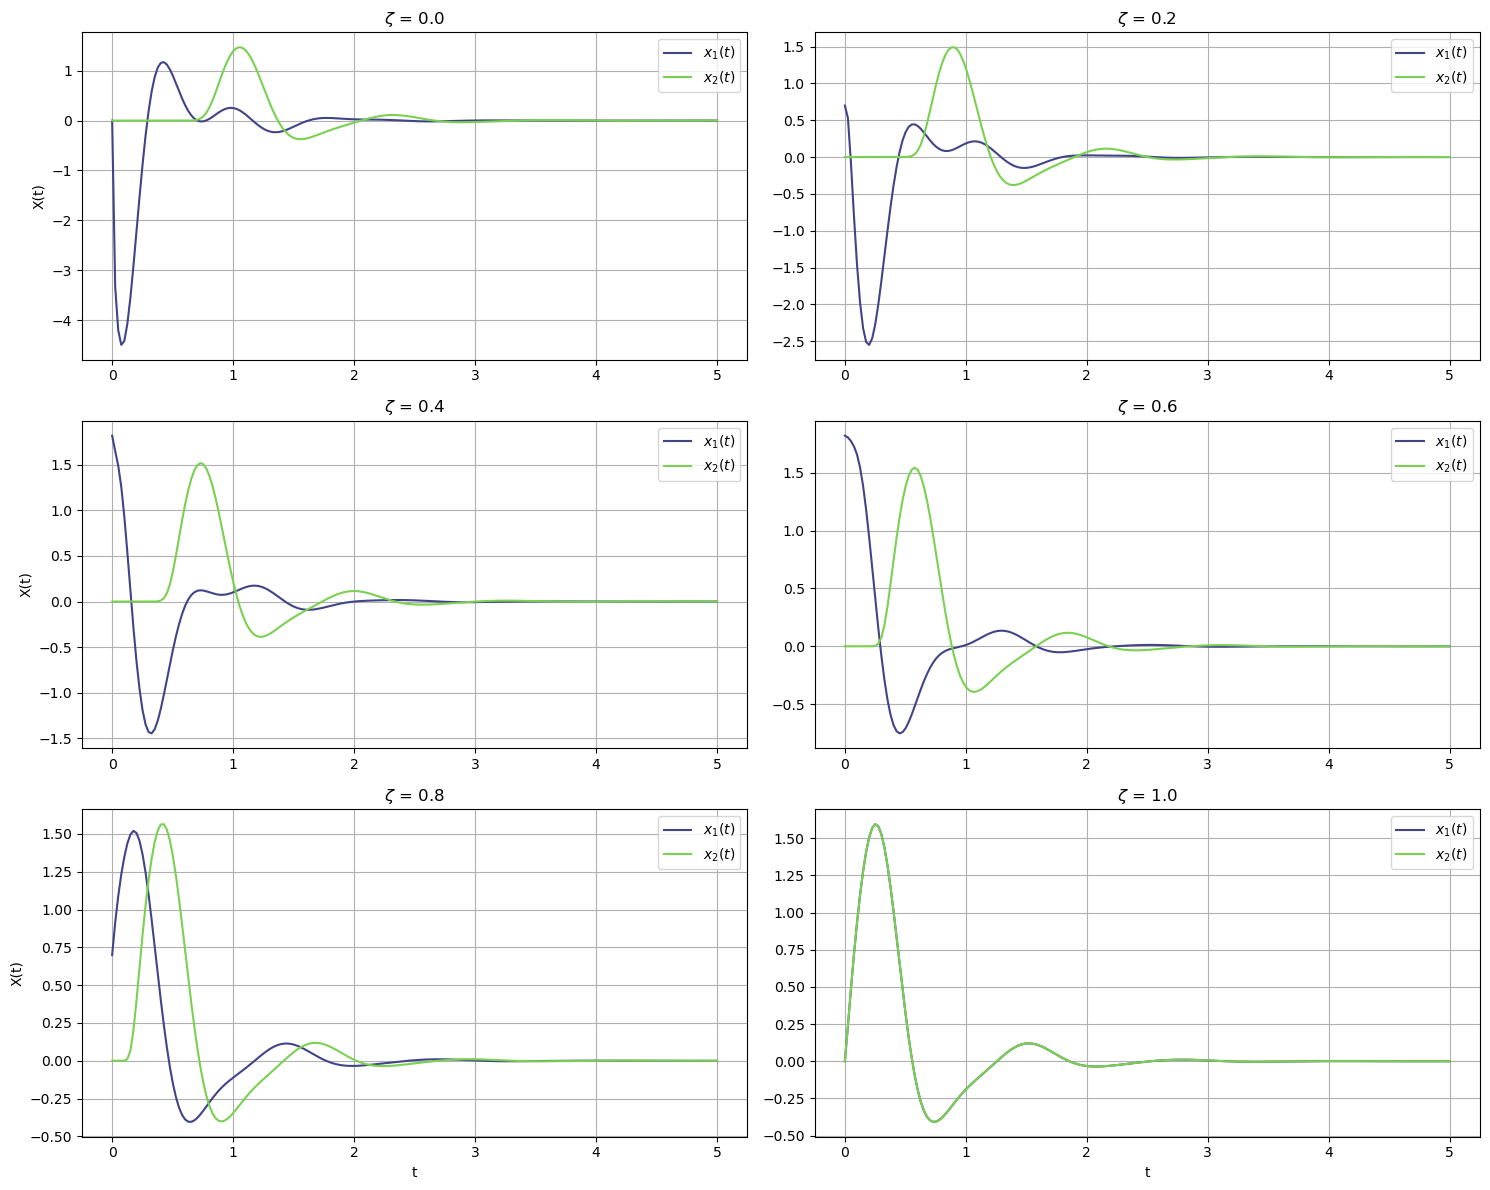
\includegraphics[width=0.8\textwidth]{Figures/2D_xt_k7.png}
    \caption{2D cross-section plots of the full-state feedback input response at various $\zeta$ positions, utilizing the feedback gain obtained in Figure~\ref{fig:k_7}.}
    \label{fig:2D_xt_k7}
\end{figure}

\begin{figure}[!htbp]
    \centering
    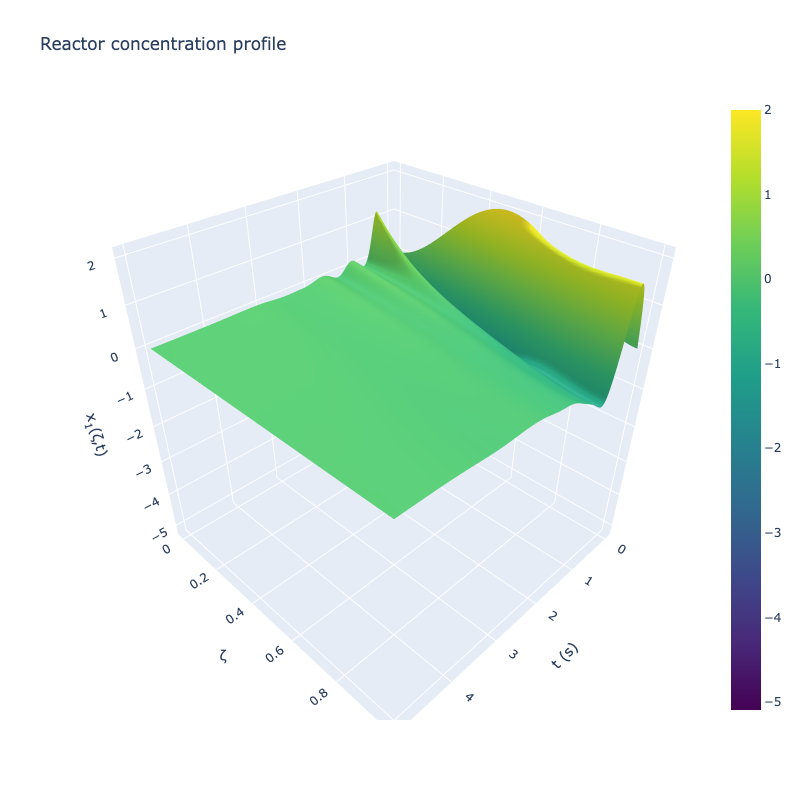
\includegraphics[width=0.8\textwidth,trim=0 0 100 0,clip]{Figures/3D_x1_L_k7.png}
    \caption{Input response of the system under observer-based output feedback control given by Equation~(\ref{eq:observer_ss}), utilizing the observer gain obtained in Figure~\ref{fig:L_modes} and the feedback gain obtained in Figure~\ref{fig:k_7}.}
    \label{fig:3D_x1_L_k7}
\end{figure}

\begin{figure}[!htbp]
    \centering
    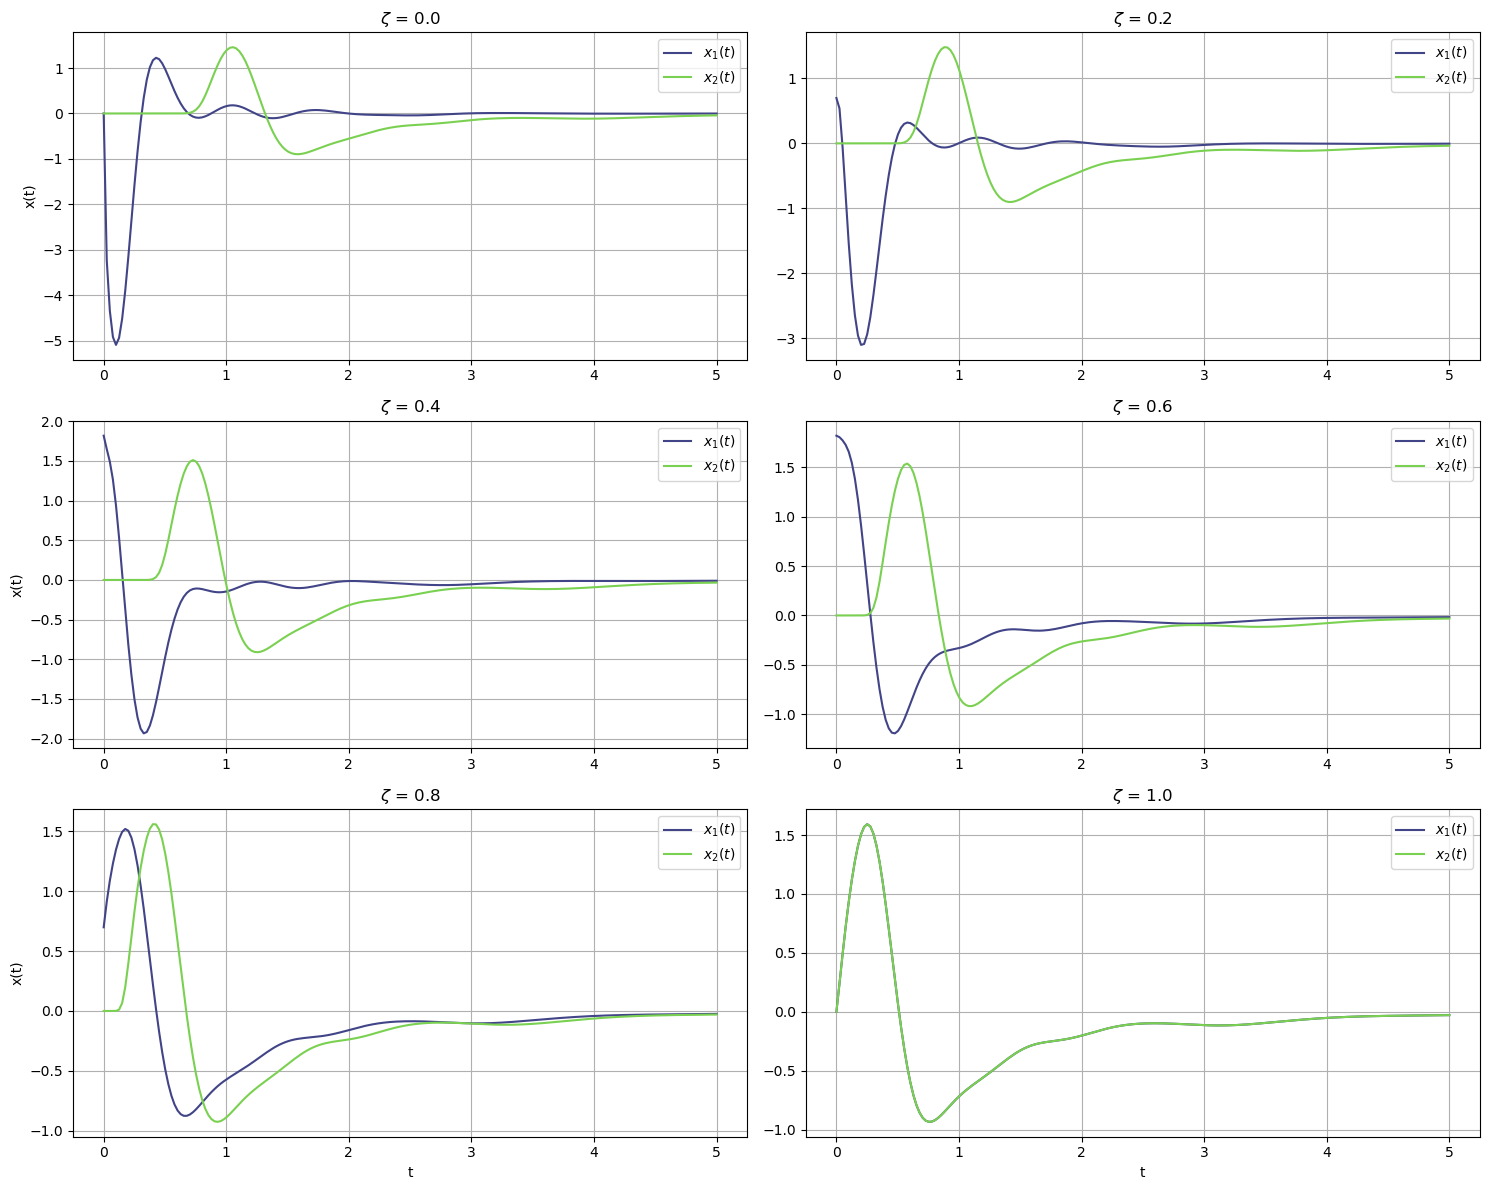
\includegraphics[width=0.8\textwidth]{Figures/2D_xt_L_k7.png}
    \caption{2D cross-section plots of the input response at various $\zeta$ positions, utilizing the observer gain obtained in Figure~\ref{fig:L_modes} and the feedback gain obtained in Figure~\ref{fig:k_7}.}
    \label{fig:2D_xt_L_k7}
\end{figure}

\begin{figure}[!htbp]
    \centering
    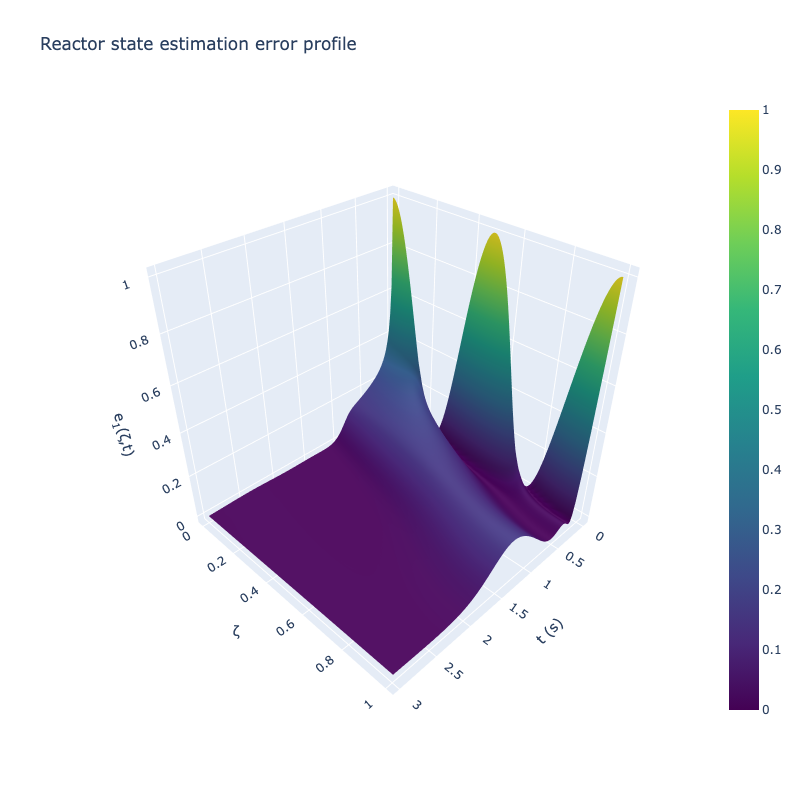
\includegraphics[width=0.8\textwidth,trim=0 0 100 0,clip]{Figures/3D_e1_L_k7.png}
    \caption{Error dynamics of the observer-based regulator utilizing the observer gain obtained in Figure~\ref{fig:L_modes} and the feedback gain obtained in Figure~\ref{fig:k_7}.}
    \label{fig:3D_e1_L_k7}
\end{figure}

\begin{figure}[!htbp]
    \centering
    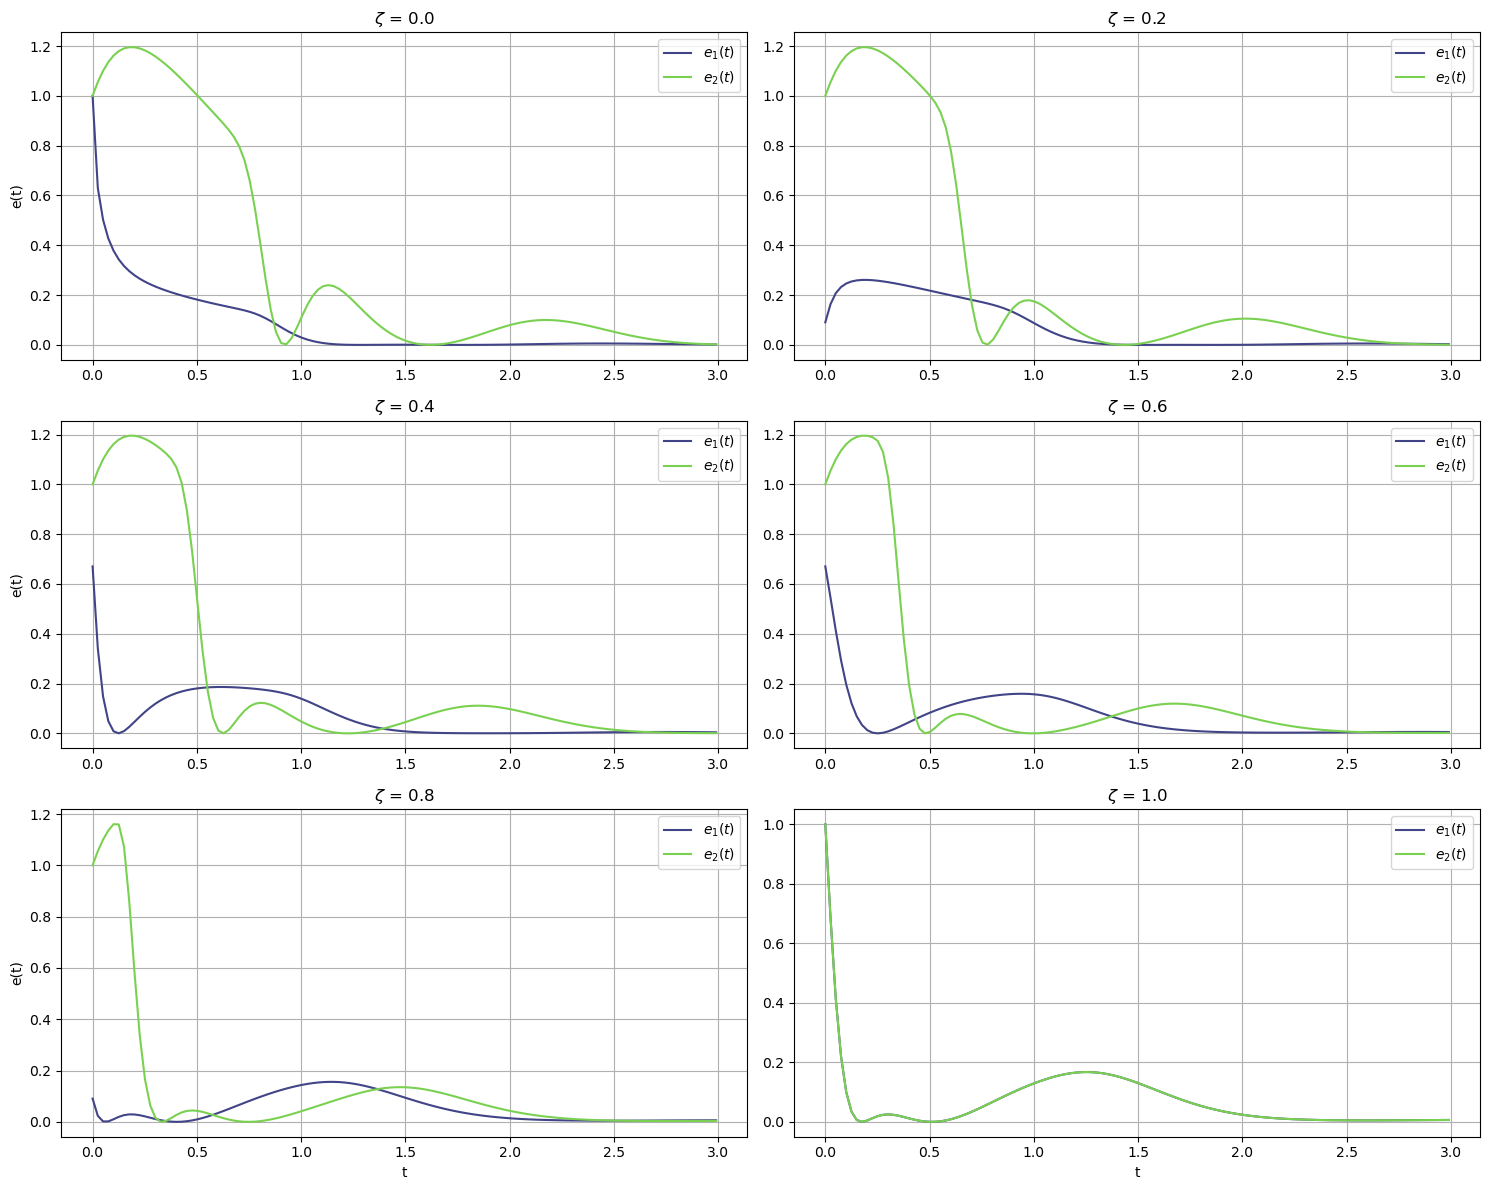
\includegraphics[width=0.8\textwidth]{Figures/2D_et_L_k7.png}
    \caption{2D cross-section plots of the error dynamics of the observer-based regulator at various $\zeta$ positions, utilizing the observer gain obtained in Figure~\ref{fig:L_modes} and the feedback gain obtained in Figure~\ref{fig:k_7}.}
    \label{fig:2D_et_L_k7}
\end{figure}
